%%%%%%%% CS725 2026 PROJECT FINAL REPORT %%%%%%%%%%%%%%%%%

\documentclass{article}

\usepackage{microtype}
\usepackage{graphicx}
\usepackage{subcaption}
\usepackage{booktabs}
\usepackage{hyperref}

\newcommand{\theHalgorithm}{\arabic{algorithm}}

\usepackage[preprint]{icml2026}
% no notice line in the first-page footer
\makeatletter\renewcommand{\Notice@String}{}\makeatother

\usepackage{amsmath}
\usepackage{amssymb}
\usepackage{mathtools}
\usepackage{amsthm}
\usepackage{multirow}
\usepackage{array}
\usepackage{float}
\usepackage{xcolor}
\usepackage{tikz}
\usetikzlibrary{positioning,arrows.meta}
\usepackage[capitalize,noabbrev]{cleveref}

\newcommand{\uhat}{\hat{u}}
\newcommand{\gapnorm}{\lVert\Delta\rVert}

\icmltitlerunning{Does Closing the Modality Gap Help Hard-Negative-Trained CLIP?}

\begin{document}

\twocolumn[
  \icmltitle{Does Closing the Modality Gap Help Hard-Negative-Trained CLIP?}

  \icmlsetsymbol{equal}{*}

  \begin{icmlauthorlist}
    \icmlauthor{Viren Mehta}{}
    \icmlauthor{Shrey Patel}{}
    \icmlauthor{Lavanay Thakral}{}
    \icmlauthor{Yash Chopra}{}
  \end{icmlauthorlist}

  \icmlkeywords{CLIP, modality gap, hard negatives, compositionality, NegCLIP}

  \vskip 0.3in
]

\makeatletter\global\icml@noticeprintedtrue\makeatother % no affiliation/notice footnote

\begin{abstract}
Closing the modality gap of CLIP after training has been proposed as a way to make it more robust at no cost in accuracy. We test this on CLIP ViT-B/32 fine-tuned on COCO with hard negatives, using 30 fine-tuning runs (five configurations, three learning rates, three seeds), four ways of shifting the embeddings, and COCO retrieval, ARO and SugarCrepe with and without embedding noise. Closing the gap after training lowers retrieval for every model and lowers COCO-Order accuracy by up to 0.38 for models trained with hard captions, and the loss is largest at the lowest learning rate, where fine-tuning barely moves the gap. Re-normalisation turns the shift into the removal of each caption's coordinate along the gap direction, which hard-caption models use to rank captions. A model trained with a penalty that closes the gap keeps or improves its compositional accuracy.
\end{abstract}

%=====================================================================
\section{Introduction}
\label{sec:intro}

CLIP \citep{radford2021clip} maps images and captions into a shared 512-dimensional space with two encoders trained by a contrastive loss. Although the loss rewards matched pairs for being close, the two modalities never mix: image embeddings and text embeddings occupy two narrow cones separated by a large offset, the \emph{modality gap} \citep{liang2022gap}. If this offset is a constant vector orthogonal to how embeddings vary, removing it after training should make CLIP more robust to perturbations without changing clean accuracy.

A separate weakness of CLIP is that it behaves like a bag of words. It scores ``the horse is eating the grass'' and ``the grass is eating the horse'' almost equally \citep{yuksekgonul2023bow}. NegCLIP addresses this by fine-tuning on COCO with \emph{hard negative captions} (word-swapped versions of each caption) and \emph{hard negative images} (visually similar images), which raises word-order accuracy on COCO-Order from 0.46 to about 0.86.

Hard negative captions sit very close to the true caption in text space, so a post-hoc shift of text embeddings could interact with exactly the fine distinctions that hard-negative training creates. We ask: \textbf{does closing the modality gap help hard-negative-trained CLIP, and does hard-negative training change the gap?} We test three hypotheses:
\textbf{H1}, hard-negative training changes the gap;
\textbf{H2}, as for CLIP, closing the gap improves robustness without hurting clean accuracy;
\textbf{H3}, since image-to-text benchmarks compare captions of the same image, a uniform shift of the text embeddings barely changes which caption wins.

Our contributions are:
(i) a grid of 30 fine-tuning runs separating hard negative images, hard negative captions, batch size and learning rate;
(ii) a post-hoc shift study over 8 models, 4 shift modes, 5 benchmarks and 4 noise levels, repeated on all 30 runs to measure the effect of the learning rate;
(iii) a mechanism: closing the gap removes each caption's coordinate along the gap direction, which hard-caption models use;
(iv) a test of closing the gap during training instead, which does not hurt compositional accuracy.

%=====================================================================
\section{Related Work}
\label{sec:related}

\textbf{Contrastive learning.}
InfoNCE \citep{oord2018cpc} pulls positive pairs together and pushes negatives apart; CLIP \citep{radford2021clip} applies it across images and text.

\textbf{The modality gap.}
\citet{liang2022gap} found that the gap appears at random initialisation, because each encoder maps its inputs into its own cone, and that contrastive training preserves it; shifting embeddings along it changes zero-shot accuracy and fairness. If the gap is orthogonal to the embedding variation, closing it should improve robustness to embedding perturbations at no clean cost; we test this on compositional models.

\textbf{Compositionality.}
The ARO benchmark \citep{yuksekgonul2023bow} tests relations, attributes and word order, and NegCLIP fine-tunes CLIP with hard negatives to solve it. SugarCrepe \citep{hsieh2023sugarcrepe} replaces ARO's often ungrammatical negatives with fluent ones, because a text-only model can solve many ARO cases. \citet{kamath2024hardpositive} show that hard-negative models can over-react to harmless rewordings. This work connects the two lines of research: it measures how hard-negative training changes the gap, and how closing the gap changes compositional accuracy.

%=====================================================================
\section{Methodology}
\label{sec:method}

\textbf{Models.}
All models are OpenCLIP ViT-B/32 with QuickGELU activations, initialised from OpenAI CLIP.\footnote{The ARO code evaluates NegCLIP with standard GELU, which raises its COCO-Order score from 0.825 to 0.868 (\cref{app:sanity}).} Besides CLIP and the released NegCLIP checkpoint, we fine-tune five configurations on the NegCLIP training split of COCO: \emph{FT plain} (256 images per batch, no hard negatives), \emph{FT + hard captions} (256 images), \emph{FT + hard images} (512 images), the \emph{FT NegCLIP recipe} with both (512 images), and \emph{FT plain, batch 512}. \emph{FT plain, batch 512} is a control we added for the final round: hard negative images double the number of images per batch, so this run tells a harder batch apart from a bigger one.

\textbf{Fine-tuning.}
We re-implemented the NegCLIP training code in a single script. A batch of $N{=}256$ items holds the images $[I, I_{\text{hard}}]$ and the texts $[T, T(I_{\text{hard}}), T_{\text{neg}}, T_{\text{neg}}(I_{\text{hard}})]$, and the loss is
\begin{equation}
\mathcal{L} = \tfrac{1}{2}\big[\mathrm{CE}(\text{img}\times\text{all texts}) + \mathrm{CE}(\text{texts}_{1:|\text{img}|}\times\text{img})\big],
\label{eq:loss}
\end{equation}
so negative captions compete only in the image-to-text direction. All runs use 5 epochs, AdamW with weight decay 0.2, a cosine schedule with 50 warm-up steps and fp16. Each configuration is trained at learning rates $\{10^{-5}, 5{\times}10^{-6}, 10^{-6}\}$ with seed 0, and the four main configurations again at $5{\times}10^{-6}$ and $10^{-6}$ with seeds 1 and 2. This gives 30 runs; the batch-512 control was run at the two lower rates. After every epoch we record the validation gap and Recall@1.

\textbf{Measuring the gap.}
For $L_2$-normalised image embeddings $x_i$ and text embeddings $y_i$ we use the gap vector of \citet{liang2022gap},
\begin{equation}
\Delta = \tfrac{1}{n}\textstyle\sum_i x_i - \tfrac{1}{n}\sum_i y_i, \qquad \uhat = \Delta/\gapnorm ,
\end{equation}
and report $\gapnorm$, the cosine between the two centroids, the fraction of each modality's variance along $\uhat$ (a random direction gets $1/512$) and the linear separability of the two modalities.

\textbf{Shifting the gap.}
$\Delta$ is fitted on COCO val and applied unchanged to every test set. With $\mathcal{N}(v)=v/\lVert v\rVert$ and shift strength $\alpha$ ($\alpha{=}1$ closes the gap before re-normalisation, $\alpha{<}0$ widens it) we use four modes:
\begin{align}
\textit{text:}\ \ & y' = \mathcal{N}(y+\alpha\Delta) \\
\textit{both:}\ \ & x' = \mathcal{N}(x-\tfrac{\alpha}{2}\Delta),\ y' = \mathcal{N}(y+\tfrac{\alpha}{2}\Delta) \\
\textit{norenorm:}\ \ & y' = y+\alpha\Delta \label{eq:norenorm}\\
\textit{orth:}\ \ & y' = \mathcal{N}\big(y - (y^\top\uhat - \overline{y^\top\uhat})\,\uhat + \alpha\Delta\big) \label{eq:orth}
\end{align}
\emph{norenorm} and \emph{orth} are controls. \emph{norenorm} adds the same constant $\alpha x^\top\Delta$ to the score of every caption of an image, so it cannot change any image-to-text ranking. \emph{orth} first removes each caption's own deviation along $\uhat$, which makes $\Delta$ exactly orthogonal to the text variation. At $\alpha{=}0$ it applies no shift and only removes that deviation. Besides an $\alpha$ sweep from $-0.5$ to $1$, we solve for $\alpha$ by bisection so that the remaining gap on COCO val equals 0.6, 0.4, 0.2 or 0.1, which compares models at equal remaining gap.

\textbf{Evaluation.}
We report COCO 5k image$\to$text and text$\to$image Recall@1 on the Karpathy test split, ARO COCO-Order, VG-Relation and VG-Attribution \citep{yuksekgonul2023bow} (macro accuracy for the VG tasks\footnote{Mean of the per-relation or per-attribute accuracies, so frequent relations do not dominate.}), and SugarCrepe \citep{hsieh2023sugarcrepe} per subset. For robustness, Gaussian noise of expected norm $\sigma\in\{0.25, 0.5, 1\}$ is added to both modalities after the shift and the embeddings are re-normalised (3 noise seeds). Every model is encoded once and all shifts run on cached embeddings. Data splits, implementation details and compute are in \cref{app:data,app:impl}.

%=====================================================================
\section{Experiments}
\label{sec:exp}

Our pipeline reproduces the published numbers we could check: CLIP's gap (0.832 vs 0.82), CLIP's COCO Recall@1 (0.502 vs 0.502), and our NegCLIP recipe matches the released checkpoint on all three ARO tasks to within 0.013 (\cref{app:sanity}).

\subsection{Hard-Negative Training and the Gap}

\begin{figure}[t]
\begin{center}
\centerline{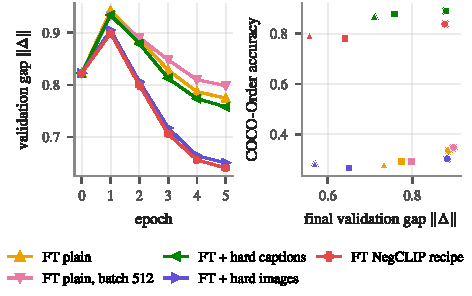
\includegraphics[width=\columnwidth]{figs/training_gap}}
\caption{Left: validation gap $\gapnorm$ (distance between the image and text centroids on COCO val) after each epoch, learning rate $5{\times}10^{-6}$. Right: COCO-Order accuracy (chance 0.2) against the final gap for every seed-0 run; marker shape gives the learning rate (circle $10^{-6}$, square $5{\times}10^{-6}$, triangle $10^{-5}$).}
\label{fig:training}
\end{center}
\vskip -0.3in
\end{figure}

\textbf{Hard negative images shrink the gap; batch size does not.}
Every run first widens the gap in epoch 1 (0.82 to 0.89--0.96) and then shrinks it (\cref{fig:training}, left). At $5{\times}10^{-6}$ the final gap is 0.650 with hard images and 0.640 with the NegCLIP recipe, against 0.775 for plain fine-tuning and 0.758 with hard captions; at $10^{-5}$ the order is the same. The batch-512 control ends at 0.799, so batch size does not explain the effect. At $10^{-6}$ all runs end near 0.88, so the learning rate sets how far the gap moves at all.

\begin{table}[t]
\caption{Clean accuracy at two learning rates (lr), mean over 3 seeds (batch 512: one seed); the standard deviation over seeds is at most 0.007 for every entry (\cref{app:train}). C-Ord: COCO-Order accuracy (chance 0.2). VG-R, VG-A: VG-Relation and VG-Attribution macro accuracy (chance 0.5). R@1: COCO 5k image$\to$text Recall@1. NegCLIP (rel.): released checkpoint. Bold: best fine-tuned model per column and lr.}
\label{tab:matched}
\begin{center}
\begin{small}
\setlength{\tabcolsep}{5pt}\renewcommand{\arraystretch}{1.1}
\begin{tabular}{llcccc}
\toprule
Model & lr & C-Ord & VG-R & VG-A & R@1 \\
\midrule
CLIP & -- & .472 & .638 & .632 & .502 \\
NegCLIP (rel.) & -- & .825 & .838 & .721 & .593 \\
\midrule
FT plain & 1e-6 & .333 & .591 & .650 & .614 \\
FT batch 512 & 1e-6 & .347 & .602 & .653 & .615 \\
FT + hard cap. & 1e-6 & \textbf{.890} & \textbf{.856} & \textbf{.729} & .593 \\
FT + hard img. & 1e-6 & .301 & .553 & .648 & .607 \\
FT NegCLIP & 1e-6 & .838 & .841 & .724 & .595 \\
\midrule
FT plain & 5e-6 & .284 & .545 & .643 & .616 \\
FT batch 512 & 5e-6 & .292 & .556 & .643 & .623 \\
FT + hard cap. & 5e-6 & \textbf{.877} & \textbf{.863} & \textbf{.736} & .601 \\
FT + hard img. & 5e-6 & .262 & .536 & .630 & .586 \\
FT NegCLIP & 5e-6 & .777 & .845 & .719 & .571 \\
\bottomrule
\end{tabular}
\end{small}
\end{center}
\vskip -0.2in
\end{table}

\textbf{Compositional skill comes from hard captions.}
Only the two configurations with hard captions become compositional (\cref{tab:matched}). Hard captions alone are the best model at every learning rate, ahead of the released NegCLIP (COCO-Order 0.87--0.89 vs 0.825), and adding hard images to them lowers COCO-Order (0.890 to 0.838 at $10^{-6}$, 0.877 to 0.777 at $5{\times}10^{-6}$). Plain COCO fine-tuning improves retrieval but makes the model less order-sensitive than CLIP. The seed standard deviation is at most 0.007, 10--60 times smaller than the differences between configurations, and the ranking is the same at all three learning rates (\cref{app:train}). \Cref{fig:training} (right) puts these together: runs with hard captions score 0.78--0.89 on COCO-Order at every gap from 0.56 to 0.88, and runs without them score 0.27--0.35 over the same range. \textbf{The size of the gap does not predict compositional skill.}

\subsection{Closing the Gap Post Hoc}

\begin{figure*}[t]
\begin{center}
\centerline{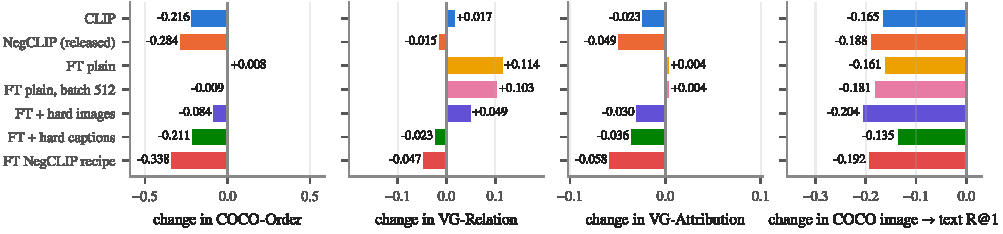
\includegraphics[width=\textwidth]{figs/closing_bars}}
\caption{Change in clean accuracy (shifted minus unshifted) when the text embeddings are moved along $\Delta$ until the remaining gap on COCO val is 0.10 (from 0.76--0.90). One bar per model, using the selected checkpoint of each configuration; negative values mean that closing the gap hurts.}
\label{fig:closing}
\end{center}
\vskip -0.25in
\end{figure*}

\Cref{fig:closing} shows the change in accuracy when the gap is closed to 0.10. For the selected checkpoints, every model trained with hard captions loses 0.21--0.34 on COCO-Order and 0.04--0.06 on VG-Attribution; our NegCLIP recipe falls from 0.838 to 0.500. Retrieval drops by 0.13--0.20 Recall@1 for every model. The only gains are on VG-Relation and only for models without hard captions (FT plain $+0.114$, batch 512 $+0.103$), which start well below CLIP there. The symmetric \emph{both} shift hurts more than the text shift, and widening the gap changes accuracy by at most 0.02 (\cref{app:shift}). This rejects H2 on clean data.

\textbf{The learning rate sets the size of the loss.} We repeated the shift on all 30 runs (\cref{app:lr}). The loss is largest at $10^{-6}$, where fine-tuning leaves the gap near 0.88: COCO-Order falls by 0.38 for FT + hard captions and 0.34 for the NegCLIP recipe, and Recall@1 by 0.18--0.21 for every configuration. At $10^{-5}$, where the gap ends at 0.56--0.73, the loss is 0.12 for hard captions, the NegCLIP recipe changes by $+0.01$, and Recall@1 falls by only 0.04--0.12. Seeds differ by at most 0.01. The more fine-tuning shrinks the gap, the less the models depend on its direction.

\subsection{Why Closing the Gap Hurts}

The \emph{norenorm} shift (\cref{eq:norenorm}) leaves every accuracy unchanged to four decimals for all 8 models, so any effect of the shift comes from re-normalisation. Write a caption as $y = y_\perp + (m+d)\,\uhat$, where $m$ is the mean projection of all captions on $\uhat$ and $d$ is the caption's own deviation. After the shift,
\begin{equation}
s'(x,y) = \frac{x^\top y + \alpha\,x^\top\Delta}{\sqrt{1 + 2\alpha\gapnorm(m+d) + \alpha^2\gapnorm^2}} .
\label{eq:score}
\end{equation}
The numerator gains a constant that is shared by all captions, and the denominator differs between captions only through $d$. Closing the gap therefore re-weights captions by their position along $\uhat$. The \emph{orth} control at $\alpha{=}0$ (\cref{eq:orth}) applies no shift and only removes $d$, and it reproduces the gap-closing change almost exactly (\cref{fig:app_mech}): $-0.327$ vs $-0.327$ for released NegCLIP on COCO-Order, $-0.364$ vs $-0.385$ for our NegCLIP recipe, $-0.223$ vs $-0.231$ for CLIP, and $+0.143$ vs $+0.125$ for FT plain on VG-Relation. \textbf{Closing the gap amounts to deleting one direction from the text embeddings.}


\textbf{The gap direction is special.} It holds only about 0.7\% of the text variance, so it is nearly orthogonal to the text variation, yet removing it costs hard-caption models 0.28--0.36 on COCO-Order and 0.06--0.07 on VG-Attribution. Removing any of 20 random directions changes accuracy by at most 0.019 on any benchmark, and removing the top text principal component, which holds about 7 times more variance than $\uhat$, costs only 0.02--0.08 on COCO-Order (\cref{app:extra}). The coordinate $d$ alone already separates true captions from their negatives: for released NegCLIP the true COCO-Order caption has the largest $d$ of the five options in 61\% of cases (chance 20\%), and the probability that $d_{\text{true}} > d_{\text{neg}}$ is 0.79--0.83 for hard-caption models against 0.42 for FT plain. Across all 32 model--benchmark pairs this probability predicts the effect of removing $d$ ($r=-0.88$, \cref{fig:probe}): where the true caption sits higher on $\uhat$, closing the gap hurts; where the negative does, as for FT plain on VG-Relation, it helps. H3 holds only without re-normalisation. $\uhat$ is also not a naturalness direction (\cref{app:nat}).

\begin{figure}[t]
\begin{center}
\centerline{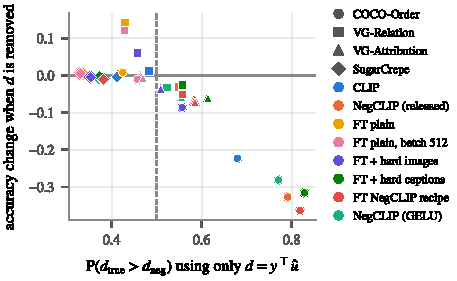
\includegraphics[width=\columnwidth]{figs/x_probe_vs_removal}}
\caption{One point per model and benchmark. x: fraction of (true, negative) caption pairs in which the true caption has the larger coordinate $d=y^\top\uhat$ along the gap direction (0.5, dashed: no information). y: accuracy change when $d$ is removed from every caption (\emph{orth}, $\alpha{=}0$). Pearson $r=-0.88$.}
\label{fig:probe}
\end{center}
\vskip -0.3in
\end{figure}

\subsection{SugarCrepe and Embedding Noise}

Hard captions lift the SugarCrepe swap subsets (swap-att 0.70 to 0.78, swap-obj 0.67 to 0.78); FT + hard captions has the best mean over subsets (0.837, released NegCLIP 0.829, CLIP 0.739). Closing the gap helps add-att ($+0.09$ to $+0.22$) and add-obj ($+0.04$ to $+0.06$) and hurts the replace and swap subsets ($-0.03$ to $-0.11$), so the pooled score barely moves (\cref{app:sugarcrepe}). The probe explains this too: in the add subsets the longer negative sits higher on $\uhat$ than the positive in 76--98\% of cases. Under embedding noise the harm shrinks (our NegCLIP recipe: $-0.338$ on COCO-Order at $\sigma{=}0$, $-0.060$ at $\sigma{=}1$), and at $\sigma{=}0.5$ closing the gap gives every model $+0.03$ to $+0.05$ on SugarCrepe (\cref{app:noise}). The benefit predicted by H2 thus appears only under noise and is no larger for hard-negative models.

\subsection{Closing the Gap During Training}

\begin{table}[t]
\caption{Fine-tuning with the penalty $\lambda\lVert\bar x-\bar y\rVert^2$ added to the loss, where $\bar x,\bar y$ are the batch means of the image and matched-caption embeddings (lr $5{\times}10^{-6}$, seed 0; $\lambda{=}0$: no penalty). gap: final validation gap $\gapnorm$. Other columns as in \cref{tab:matched}.}
\label{tab:gapreg}
\begin{center}
\begin{small}
\setlength{\tabcolsep}{3.5pt}
\begin{tabular}{lccccccc}
\toprule
Config. & $\lambda$ & gap & C-Ord & VG-R & VG-A & R@1 \\
\midrule
FT + hard cap. & 0 & .758 & .878 & .860 & .738 & .599 \\
 & 1 & .038 & .907 & .852 & .732 & .587 \\
 & 10 & .030 & \textbf{.915} & \textbf{.867} & .727 & .583 \\
\midrule
FT NegCLIP & 0 & .640 & .781 & .847 & .723 & .574 \\
 & 10 & .033 & \textbf{.862} & .847 & .704 & .566 \\
\midrule
FT plain & 0 & .775 & .291 & .542 & .647 & .618 \\
 & 10 & .030 & .292 & \textbf{.610} & .631 & .599 \\
\bottomrule
\end{tabular}
\end{small}
\end{center}
\vskip -0.2in
\end{table}

If the damage comes from deleting a coordinate the model has learned to use, a model trained with a closed gap should not suffer. We added $\lambda\lVert\bar x-\bar y\rVert^2$, the squared distance between the batch means of image and matched-text embeddings, to \cref{eq:loss}. The gap falls below 0.06 within one epoch and ends at 0.03--0.04 (\cref{tab:gapreg}, \cref{app:gapreg}). Compositional accuracy does not drop: COCO-Order rises from 0.878 to 0.915 with hard captions and from 0.781 to 0.862 with the NegCLIP recipe, and VG-Relation of FT plain rises from 0.542 to 0.610, at a cost of 0.01--0.02 Recall@1 and up to 0.02 on VG-Attribution. In these models removing $d$ changes COCO-Order by less than 0.01, so the compositional information no longer sits on the gap direction.

%=====================================================================
\section{Conclusion}
\label{sec:conclusion}

Closing the modality gap after training does not help hard-negative-trained CLIP: at the selected learning rates it costs every model trained with hard captions 0.21--0.34 on COCO-Order and every model retrieval accuracy, and helps only under strong embedding noise (H2 rejected). Re-normalisation turns the shift into the removal of each caption's coordinate along the gap direction, a coordinate that hard-caption models use to rank true captions above their negatives (H3 rejected for order and attribute tasks). The loss shrinks as the learning rate grows (0.38 at $10^{-6}$, at most 0.12 at $10^{-5}$). Hard negative images shrink the gap during training while hard negative captions give compositional skill (H1 partly supported). A model trained with a penalty that keeps its gap near 0.03 keeps or improves its compositional accuracy.

\bibliography{references}
\bibliographystyle{icml2026}

%=====================================================================
\newpage % in two-column mode: start the right column
\section*{Team Contribution}

\begin{itemize}
\item \textbf{Viren Mehta}: Designed the experiments, implemented the proposed approach, evaluated experimental results, and reviewed relevant research literature.
\item \textbf{Shrey Patel}: Undertook dataset preparation, conducted a comprehensive literature review, investigated research papers and their practical applications, and replicated existing research papers.
\item \textbf{Lavanay Thakral}: Examined relevant research papers, developed potential extensions to existing methodologies, and analyzed experimental results.
\item \textbf{Yash Chopra}: Explored and assessed the dataset, developed project presentations, and performed comparative evaluations of existing research papers and methods.
\end{itemize}

\section*{AI Usage}

AI tools, including ChatGPT, were used to assist with code formatting, debugging, graph generation, and report formatting. They also supported the implementation and replication of results from the research paper ``Mind the Gap: Understanding the Modality Gap in Multi-modal Contrastive Representation Learning'' \citep{liang2022gap}.


%=====================================================================
% APPENDIX
%=====================================================================
\clearpage
\appendix

\section{Data and Implementation}
\label{app:data}\label{app:impl}

\textbf{Data.} Fine-tuning uses the NegCLIP training split of COCO \citep{lin2014coco} (109,468 images, each with 1 caption, 1--6 hard negative captions and 3 neighbour images). COCO Karpathy val (5,000 images, 25,010 captions) is used for checkpoint selection, the per-epoch gap and fitting $\Delta$; Karpathy test (same size) for retrieval and gap metrics. ARO COCO-Order has 25,010 cases with 4 shuffled negatives, VG-Relation 23,937 and VG-Attribution 28,748 cases, and SugarCrepe 7,511 cases in seven subsets. Val and test share no image with the training split (checked by file name). COCO-Order negatives are drawn once with seed 0 and cached, so every model and shift is scored on the same negatives.

\textbf{Implementation.} Every model is built as OpenCLIP \texttt{ViT-B-32-quickgelu}; the weights of the released NegCLIP training checkpoint were extracted with PyTorch's restricted loader. Training: AdamW with $\beta=(0.9, 0.98)$, weight decay 0.2 except on gains, biases and the logit scale, cosine schedule, fp16, RandomResizedCrop with scale 0.9--1.0, and one hard negative caption and one neighbour image drawn per item per epoch. The selected checkpoint of each configuration is the learning rate with the best final validation Recall@1 ($5{\times}10^{-6}$ for FT plain and FT + hard captions, $10^{-6}$ for the others). The text encoder is run only up to the longest caption of each batch, which gives identical embeddings (difference below $3{\times}10^{-7}$) five times faster. Training ran on a shared server with four 48\,GB GPUs (about 16 GPU-hours for the 30 runs; one epoch 219--411\,s); shifts and evaluation ran on cached embeddings on a CPU pool.

\section{Sanity Checks}
\label{app:sanity}

Our pipeline gives a CLIP gap of 0.832 on COCO (published 0.82), CLIP COCO Recall@1 of 0.502 / 0.302 (image$\to$text / text$\to$image; published 0.502 / 0.304) and CLIP VG-Relation / VG-Attribution / COCO-Order of 0.638 / 0.632 / 0.472 (published 0.59--0.63 / 0.62 / 0.46). Released NegCLIP scores 0.838 / 0.721 / 0.825 (published 0.81 / 0.71 / 0.86), and our NegCLIP recipe at $10^{-6}$ scores 0.840 / 0.725 / 0.838. NegCLIP was trained with QuickGELU, but the ARO code evaluates it with standard GELU. With QuickGELU it scores 0.825 on COCO-Order, with GELU 0.868, which matches the published 0.86. We use QuickGELU throughout.

\section{Training and Seeds}
\label{app:train}

\begin{table}[H]
\caption{Final-epoch validation gap $\gapnorm$ and mean Recall@1 (average of image$\to$text and text$\to$image R@1 on COCO val) for every configuration and learning rate (seed 0). --: not run.}
\label{tab:valgap}
\begin{center}
\begin{small}
\setlength{\tabcolsep}{3pt}
\begin{tabular}{lcccccc}
\toprule
& \multicolumn{3}{c}{gap} & \multicolumn{3}{c}{mean R@1} \\
lr & 1e-6 & 5e-6 & 1e-5 & 1e-6 & 5e-6 & 1e-5 \\
\midrule
FT plain & .886 & .775 & .733 & .442 & .457 & .457 \\
FT 512 & .897 & .799 & -- & .440 & .456 & -- \\
FT + cap. & .880 & .758 & .710 & .427 & .445 & .438 \\
FT + img. & .883 & .650 & .569 & .444 & .430 & .420 \\
FT NegCLIP & .877 & .640 & .557 & .437 & .420 & .412 \\
\bottomrule
\end{tabular}
\end{small}
\end{center}
\vskip -0.1in
\end{table}

At $10^{-5}$ (seed 0) COCO-Order is 0.278 for FT plain, 0.869 with hard captions, 0.282 with hard images and 0.791 for the NegCLIP recipe, so the ranking of \cref{tab:matched} holds at every learning rate. The seed standard deviation is at most 0.007 on every metric. The batch-512 control stays within 0.015 of FT plain on all clean metrics, and its gap (0.799 at $5{\times}10^{-6}$) is close to FT plain (0.775), not to FT + hard images (0.650). In every model the gap direction holds 0.2--0.4\% of the image and 0.7--0.8\% of the text variance, and the two modalities stay perfectly linearly separable.

\section{Shift Results and Mechanism}
\label{app:shift}\label{app:mechanism}

\begin{table}[H]
\caption{Accuracy change for the selected checkpoints. close: text shift to a remaining gap of 0.10. rem.\ $d$: no shift; only each caption's deviation $d$ along $\uhat$ is removed (\emph{orth}, $\alpha{=}0$). Abbreviations as in \cref{tab:matched}.}
\label{tab:closing}
\begin{center}
\begin{small}
\setlength{\tabcolsep}{2.3pt}
\begin{tabular}{lcccccc}
\toprule
& \multicolumn{2}{c}{C-Ord} & \multicolumn{2}{c}{VG-R} & VG-A & R@1 \\
Model & close & rem.\ $d$ & close & rem.\ $d$ & close & close \\
\midrule
CLIP & $-.216$ & $-.223$ & $+.017$ & $+.012$ & $-.023$ & $-.165$ \\
NegCLIP & $-.284$ & $-.327$ & $-.015$ & $-.031$ & $-.049$ & $-.188$ \\
NegCLIP GELU & $-.279$ & $-.281$ & $-.024$ & $-.032$ & $-.052$ & $-.199$ \\
FT plain & $+.008$ & $+.008$ & $+.114$ & $+.143$ & $+.004$ & $-.161$ \\
FT 512 & $-.009$ & $-.010$ & $+.103$ & $+.121$ & $+.004$ & $-.181$ \\
FT + cap. & $-.211$ & $-.316$ & $-.023$ & $-.025$ & $-.036$ & $-.135$ \\
FT + img. & $-.084$ & $-.086$ & $+.049$ & $+.061$ & $-.030$ & $-.204$ \\
FT NegCLIP & $-.338$ & $-.364$ & $-.047$ & $-.052$ & $-.058$ & $-.192$ \\
\bottomrule
\end{tabular}
\end{small}
\end{center}
\vskip -0.1in
\end{table}

\begin{figure}[H]
\begin{center}
\centerline{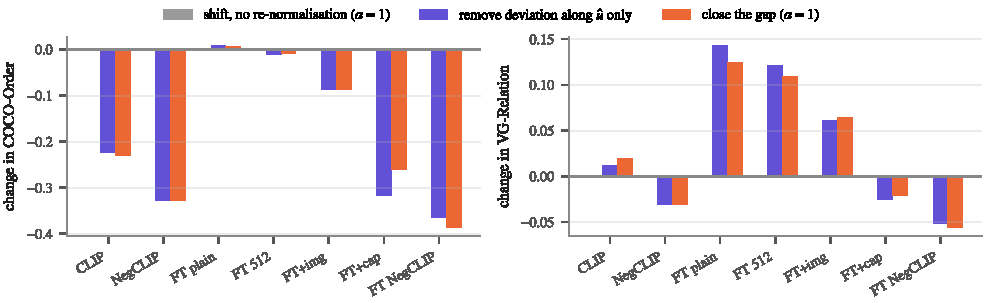
\includegraphics[width=\columnwidth]{figs/app_mechanism}}
\caption{Change in COCO-Order and VG-Relation from three interventions at $\alpha{=}1$: the shift without re-normalisation (\emph{norenorm}, grey) is zero for every model, and removing $d$ alone (\emph{orth} at $\alpha{=}0$, purple) matches closing the gap with re-normalisation (\emph{text}, orange).}
\label{fig:app_mech}
\end{center}
\vskip -0.2in
\end{figure}

For each model we ran 7 values of $\alpha$ and 4 target gaps with the mean and the coordinate-wise median gap vector in all four modes; the two estimators agree within 0.01 and the symmetric shift is always more harmful than the text shift. In float32, \emph{norenorm} flips 2 of 25,010 near-tied COCO-Order cases for CLIP, below the fourth decimal.

\section{Learning Rate and Post-Hoc Closing}
\label{app:lr}

Each of the 30 runs was encoded and shifted to a remaining gap of 0.10 (text shift), and separately had $d$ removed. \Cref{tab:lr,fig:lr} give the change, averaged over the available seeds.

\begin{table}[H]
\caption{Accuracy change for every grid run, averaged over $n$ seeds. gap: $\gapnorm$ on COCO val before the shift. close: text shift to a remaining gap of 0.10. rem.\ $d$: removal of $d$ only. Abbreviations as in \cref{tab:matched}.}
\label{tab:lr}
\begin{center}
\begin{small}
\setlength{\tabcolsep}{1.6pt}
\resizebox{\columnwidth}{!}{\begin{tabular}{llcccccccc}
\toprule
& & & & \multicolumn{2}{c}{C-Ord} & VG-R & VG-A & R@1 \\
Config. & lr & $n$ & gap & close & rem.\ $d$ & close & close & close \\
\midrule
\csname @@input\endcsname lr_table.tex
\bottomrule
\end{tabular}}
\end{small}
\end{center}
\vskip -0.1in
\end{table}

\begin{figure*}[t]
\begin{center}
\centerline{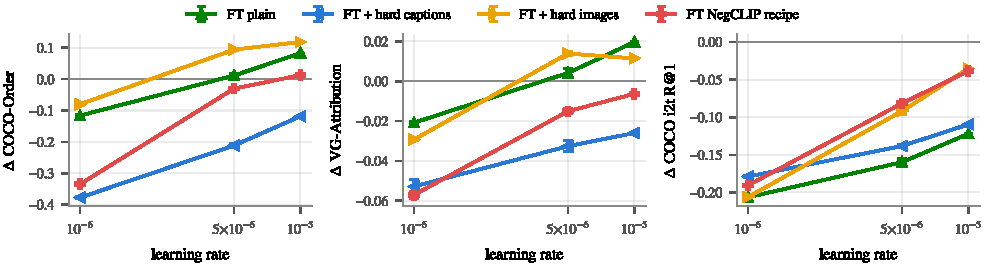
\includegraphics[width=\textwidth]{figs/lr_closing}}
\caption{Accuracy change (shifted minus unshifted) from closing the gap to 0.10 with the text shift, against the fine-tuning learning rate. Points: mean over seeds (3 at $10^{-6}$ and $5{\times}10^{-6}$, 1 at $10^{-5}$); error bars: std over seeds.}
\label{fig:lr}
\end{center}
\vskip -0.2in
\end{figure*}

\section{SugarCrepe and Noise}
\label{app:sugarcrepe}\label{app:noise}

\begin{figure}[H]
\begin{center}
\centerline{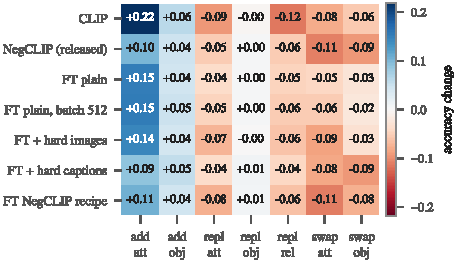
\includegraphics[width=0.9\columnwidth]{figs/sugarcrepe_delta}}
\caption{Change in SugarCrepe accuracy per subset after closing the gap (text shift, $\alpha{=}1$). add/replace/swap: how the negative caption was built; att/obj/rel: the attribute, object or relation that was changed. Blue: gain; red: loss.}
\label{fig:sugarcrepe}
\end{center}
\vskip -0.2in
\end{figure}

Plain COCO fine-tuning lifts the add and replace subsets, and only hard captions lift the swap subsets. Mean clean accuracy over subsets is 0.739 for CLIP, 0.829 for released NegCLIP and 0.837 for FT + hard captions.

\begin{table}[H]
\caption{Accuracy change from closing the gap to 0.10 when Gaussian noise of expected norm $\sigma$ is added to the image and text embeddings after the shift (mean of 3 noise seeds); $\sigma{=}0$ is the clean setting.}
\label{tab:noise}
\begin{center}
\begin{small}
\setlength{\tabcolsep}{2.4pt}
\begin{tabular}{lcccccc}
\toprule
& \multicolumn{3}{c}{COCO-Order} & \multicolumn{3}{c}{SugarCrepe} \\
Model & $\sigma{=}0$ & 0.5 & 1.0 & $\sigma{=}0$ & 0.5 & 1.0 \\
\midrule
CLIP & $-.216$ & $-.085$ & $-.034$ & $-.000$ & $+.040$ & $+.021$ \\
NegCLIP & $-.284$ & $-.124$ & $-.054$ & $-.003$ & $+.043$ & $+.022$ \\
FT plain & $+.008$ & $+.008$ & $+.002$ & $+.011$ & $+.041$ & $+.025$ \\
FT + cap. & $-.211$ & $-.136$ & $-.071$ & $+.005$ & $+.032$ & $+.021$ \\
FT + img. & $-.084$ & $-.030$ & $-.012$ & $+.001$ & $+.053$ & $+.027$ \\
FT NegCLIP & $-.338$ & $-.142$ & $-.060$ & $-.005$ & $+.045$ & $+.023$ \\
\bottomrule
\end{tabular}
\end{small}
\end{center}
\vskip -0.1in
\end{table}

\section{Analyses of the Gap Direction}
\label{app:extra}

\begin{figure*}[t]
\begin{center}
\centerline{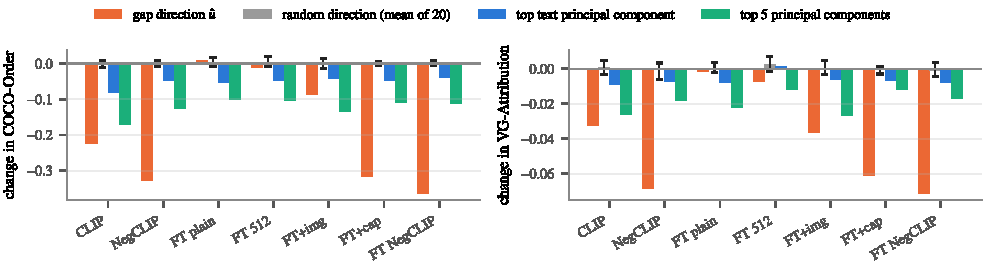
\includegraphics[width=\textwidth]{figs/x_direction_removal}}
\caption{Accuracy change from removing each caption's deviation from the benchmark mean along one direction or subspace: the gap direction $\uhat$, 20 random unit directions (bar: mean; whiskers: range) and the top 1 or 5 principal components of the COCO-val text embeddings.}
\label{fig:x_removal}
\end{center}
\vskip -0.2in
\end{figure*}

\textbf{Direction removal.} Removing the deviation along any of 20 random directions changes accuracy by at most 0.019. The top text principal component holds 4.3--5.8\% of the text variance, 6.6--7.7 times more than $\uhat$, and removing it costs 0.02--0.08 on COCO-Order; the top 5 components cost 0.06--0.17, still less than $\uhat$ alone for every hard-caption model (\cref{fig:x_removal}).

\textbf{One-coordinate probe.} The probability that the true caption has a larger $d$ than a negative is, on COCO-Order, 0.68 for CLIP, 0.79 for released NegCLIP, 0.83 for FT + hard captions, 0.82 for the NegCLIP recipe, 0.56 for FT + hard images and 0.43 for FT plain. On VG-Relation it is 0.43--0.56 and on SugarCrepe 0.33--0.41 for every model.

\textbf{Caption length.} $d$ is weakly correlated with the number of words (Spearman $\rho$ 0.09--0.20 on COCO-Order, 0.23--0.29 on SugarCrepe). In the SugarCrepe add subsets the negative is 1.1 (add-att) and 3.3 (add-obj) words longer than the positive and has the larger $d$ in 76--98\% of cases, which is why closing the gap helps these subsets. Within a subset, the length difference is only weakly related to the $d$ difference ($\rho=0.06$--$0.19$).

\textbf{Keeping $d$.} Closing the gap and then restoring each caption's deviation along $\uhat$ recovers little (released NegCLIP COCO-Order 0.541 to 0.579, against 0.825 unshifted), because each caption's score is still divided by its own norm $\lVert y+\alpha\Delta\rVert$, which depends on $d$ (\cref{eq:score}).

\textbf{Naturalness.} \label{app:nat} The Spearman correlation between $y^\top\uhat$ and GPT-2 perplexity over the 119,724 COCO-Order captions is between $-0.18$ and $+0.06$ for every model.

\section{Closing the Gap During Training}
\label{app:gapreg}

\begin{figure}[H]
\begin{center}
\centerline{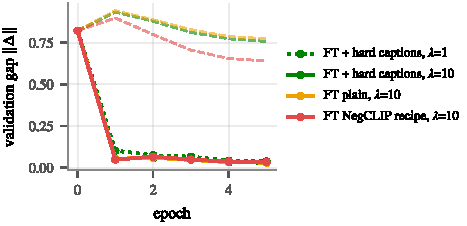
\includegraphics[width=\columnwidth]{figs/x_gapreg_curves}}
\caption{Validation gap $\gapnorm$ after each epoch with the gap penalty (solid, dotted) and without it ($\lambda{=}0$, dashed), at lr $5{\times}10^{-6}$.}
\label{fig:x_gapreg}
\end{center}
\vskip -0.2in
\end{figure}

The penalty is computed per batch over the images and their matched captions (hard negative captions excluded), with all other settings as in the main grid (lr $5{\times}10^{-6}$, seed 0). The final gap on all COCO-val captions is 0.04--0.05, and validation mean Recall@1 is 0.413--0.439 against 0.420--0.457 without the penalty. In these models removing $d$ changes COCO-Order by at most 0.009. The penalty does not improve robustness to noise: at $\sigma{=}0.5$, text$\to$image Recall@1 is 0.301 for FT + hard captions with $\lambda{=}10$ against 0.322 without it. The COCO-Order gains (0.03--0.08) are 5--10 times the seed standard deviation.

\section{Summary of Findings}
\label{app:summary}

\Cref{tab:summary} lists the three hypotheses of \cref{sec:intro}, the gap-penalty experiment, and the main evidence for each outcome.


\begin{table}[H]
\caption{Hypotheses and the evidence for each. C-Ord: COCO-Order; R@1: COCO image$\to$text Recall@1.}
\label{tab:summary}
\begin{center}
\begin{small}
\setlength{\tabcolsep}{3pt}
\begin{tabular}{@{}>{\raggedright\arraybackslash}p{0.27\columnwidth}>{\raggedright\arraybackslash}p{0.70\columnwidth}@{}}
\toprule
Hypothesis & Outcome \\
\midrule
H1: training changes the gap & Partly: hard images shrink it (0.650 vs 0.775 at $5{\times}10^{-6}$); hard captions do not. \\
H2: closing is free & Rejected: C-Ord $-0.12$ to $-0.38$ for hard-caption models, R@1 $-0.04$ to $-0.21$; gains only under noise. \\
H3: rankings are kept & Only without re-normalisation. \\
Gap penalty & No loss: C-Ord $+0.03$ to $+0.08$. \\
\bottomrule
\end{tabular}
\end{small}
\end{center}
\vskip -0.1in
\end{table}

\end{document}
